\documentclass[10pt]{standalone}
\usepackage[sc]{mathpazo}
\usepackage{commands}

\begin{document}
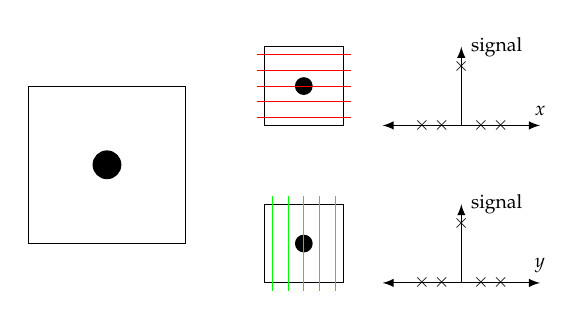
\begin{tikzpicture}
    \draw[] (0, 0) -- (2, 0) -- (2, 2) -- (0, 2) -- cycle;
    \draw[fill = black] (1, 1) circle (5pt);

    \draw[] (0+3, 0+1.5) -- (1+3, 0+1.5) -- (1+3, 1+1.5) -- (0+3, 1+1.5) -- cycle;
    \draw[fill = black] (0.5+3, 0.5+1.5) circle (3pt);
    \foreach \i in {0.1, 0.3, ..., 0.9} {
        \draw[red] (0+3-0.1, 0+1.5 + \i) -- (1+3+0.1, 0+1.5 + \i);
    }
    \draw[latex-latex] (4.5, 1.5) -- (6.5, 1.5);
    \draw[-latex] (5.5, 1.5) -- (5.5, 2.5);
    \node[above] at (6.5, 1.5) {\scriptsize $x$};
    \node[right] at (5.5, 2.5) {\scriptsize signal};
    \node[] at (5, 1.5) {\scriptsize $\times$};
    \node[] at (5.25, 1.5) {\scriptsize $\times$};
    \node[] at (5.5, 2.25) {\scriptsize $\times$};
    \node[] at (5.75, 1.5) {\scriptsize $\times$};
    \node[] at (6, 1.5) {\scriptsize $\times$};
    
    \draw[] (0+3, 0-0.5) -- (1+3, 0-0.5) -- (1+3, 1-0.5) -- (0+3, 1-0.5) -- cycle;
    \draw[fill = black] (0.5+3, 0.5-0.5) circle (3pt);
    \foreach \i in {0.1, 0.3, ..., 0.9} {
        \draw[green] (0+3+\i, 0-0.5-0.1) -- (0+3+\i, 0+1-0.5+0.1);
    }
    \draw[latex-latex] (4.5, -0.5) -- (6.5, -0.5);
    \draw[-latex] (5.5, -0.5) -- (5.5, 0.5);
    \node[above] at (6.5, -0.5) {\scriptsize $y$};
    \node[right] at (5.5, 0.5) {\scriptsize signal};
    \node[] at (5, -0.5) {\scriptsize $\times$};
    \node[] at (5.25, -0.5) {\scriptsize $\times$};
    \node[] at (5.5, 0.25) {\scriptsize $\times$};
    \node[] at (5.75, -0.5) {\scriptsize $\times$};
    \node[] at (6, -0.5) {\scriptsize $\times$};
\end{tikzpicture}
\end{document}